% Options for packages loaded elsewhere
\PassOptionsToPackage{unicode}{hyperref}
\PassOptionsToPackage{hyphens}{url}
\PassOptionsToPackage{dvipsnames,svgnames,x11names}{xcolor}
%
\documentclass[
  11pt,
  letterpaper]{article}
\usepackage{amsmath,amssymb}
\usepackage{iftex}
\ifPDFTeX
  \usepackage[T1]{fontenc}
  \usepackage[utf8]{inputenc}
  \usepackage{textcomp} % provide euro and other symbols
\else % if luatex or xetex
  \usepackage{unicode-math} % this also loads fontspec
  \defaultfontfeatures{Scale=MatchLowercase}
  \defaultfontfeatures[\rmfamily]{Ligatures=TeX,Scale=1}
\fi
\usepackage{lmodern}
\ifPDFTeX\else
  % xetex/luatex font selection
\fi
% Use upquote if available, for straight quotes in verbatim environments
\IfFileExists{upquote.sty}{\usepackage{upquote}}{}
\IfFileExists{microtype.sty}{% use microtype if available
  \usepackage[]{microtype}
  \UseMicrotypeSet[protrusion]{basicmath} % disable protrusion for tt fonts
}{}
\makeatletter
\@ifundefined{KOMAClassName}{% if non-KOMA class
  \IfFileExists{parskip.sty}{%
    \usepackage{parskip}
  }{% else
    \setlength{\parindent}{0pt}
    \setlength{\parskip}{6pt plus 2pt minus 1pt}}
}{% if KOMA class
  \KOMAoptions{parskip=half}}
\makeatother
\usepackage{xcolor}
\usepackage[margin=1in]{geometry}
\usepackage{color}
\usepackage{fancyvrb}
\newcommand{\VerbBar}{|}
\newcommand{\VERB}{\Verb[commandchars=\\\{\}]}
\DefineVerbatimEnvironment{Highlighting}{Verbatim}{commandchars=\\\{\}}
% Add ',fontsize=\small' for more characters per line
\usepackage{framed}
\definecolor{shadecolor}{RGB}{248,248,248}
\newenvironment{Shaded}{\begin{snugshade}}{\end{snugshade}}
\newcommand{\AlertTok}[1]{\textcolor[rgb]{0.94,0.16,0.16}{#1}}
\newcommand{\AnnotationTok}[1]{\textcolor[rgb]{0.56,0.35,0.01}{\textbf{\textit{#1}}}}
\newcommand{\AttributeTok}[1]{\textcolor[rgb]{0.13,0.29,0.53}{#1}}
\newcommand{\BaseNTok}[1]{\textcolor[rgb]{0.00,0.00,0.81}{#1}}
\newcommand{\BuiltInTok}[1]{#1}
\newcommand{\CharTok}[1]{\textcolor[rgb]{0.31,0.60,0.02}{#1}}
\newcommand{\CommentTok}[1]{\textcolor[rgb]{0.56,0.35,0.01}{\textit{#1}}}
\newcommand{\CommentVarTok}[1]{\textcolor[rgb]{0.56,0.35,0.01}{\textbf{\textit{#1}}}}
\newcommand{\ConstantTok}[1]{\textcolor[rgb]{0.56,0.35,0.01}{#1}}
\newcommand{\ControlFlowTok}[1]{\textcolor[rgb]{0.13,0.29,0.53}{\textbf{#1}}}
\newcommand{\DataTypeTok}[1]{\textcolor[rgb]{0.13,0.29,0.53}{#1}}
\newcommand{\DecValTok}[1]{\textcolor[rgb]{0.00,0.00,0.81}{#1}}
\newcommand{\DocumentationTok}[1]{\textcolor[rgb]{0.56,0.35,0.01}{\textbf{\textit{#1}}}}
\newcommand{\ErrorTok}[1]{\textcolor[rgb]{0.64,0.00,0.00}{\textbf{#1}}}
\newcommand{\ExtensionTok}[1]{#1}
\newcommand{\FloatTok}[1]{\textcolor[rgb]{0.00,0.00,0.81}{#1}}
\newcommand{\FunctionTok}[1]{\textcolor[rgb]{0.13,0.29,0.53}{\textbf{#1}}}
\newcommand{\ImportTok}[1]{#1}
\newcommand{\InformationTok}[1]{\textcolor[rgb]{0.56,0.35,0.01}{\textbf{\textit{#1}}}}
\newcommand{\KeywordTok}[1]{\textcolor[rgb]{0.13,0.29,0.53}{\textbf{#1}}}
\newcommand{\NormalTok}[1]{#1}
\newcommand{\OperatorTok}[1]{\textcolor[rgb]{0.81,0.36,0.00}{\textbf{#1}}}
\newcommand{\OtherTok}[1]{\textcolor[rgb]{0.56,0.35,0.01}{#1}}
\newcommand{\PreprocessorTok}[1]{\textcolor[rgb]{0.56,0.35,0.01}{\textit{#1}}}
\newcommand{\RegionMarkerTok}[1]{#1}
\newcommand{\SpecialCharTok}[1]{\textcolor[rgb]{0.81,0.36,0.00}{\textbf{#1}}}
\newcommand{\SpecialStringTok}[1]{\textcolor[rgb]{0.31,0.60,0.02}{#1}}
\newcommand{\StringTok}[1]{\textcolor[rgb]{0.31,0.60,0.02}{#1}}
\newcommand{\VariableTok}[1]{\textcolor[rgb]{0.00,0.00,0.00}{#1}}
\newcommand{\VerbatimStringTok}[1]{\textcolor[rgb]{0.31,0.60,0.02}{#1}}
\newcommand{\WarningTok}[1]{\textcolor[rgb]{0.56,0.35,0.01}{\textbf{\textit{#1}}}}
\usepackage{longtable,booktabs,array}
\usepackage{calc} % for calculating minipage widths
% Correct order of tables after \paragraph or \subparagraph
\usepackage{etoolbox}
\makeatletter
\patchcmd\longtable{\par}{\if@noskipsec\mbox{}\fi\par}{}{}
\makeatother
% Allow footnotes in longtable head/foot
\IfFileExists{footnotehyper.sty}{\usepackage{footnotehyper}}{\usepackage{footnote}}
\makesavenoteenv{longtable}
\usepackage{graphicx}
\makeatletter
\newsavebox\pandoc@box
\newcommand*\pandocbounded[1]{% scales image to fit in text height/width
  \sbox\pandoc@box{#1}%
  \Gscale@div\@tempa{\textheight}{\dimexpr\ht\pandoc@box+\dp\pandoc@box\relax}%
  \Gscale@div\@tempb{\linewidth}{\wd\pandoc@box}%
  \ifdim\@tempb\p@<\@tempa\p@\let\@tempa\@tempb\fi% select the smaller of both
  \ifdim\@tempa\p@<\p@\scalebox{\@tempa}{\usebox\pandoc@box}%
  \else\usebox{\pandoc@box}%
  \fi%
}
% Set default figure placement to htbp
\def\fps@figure{htbp}
\makeatother
\setlength{\emergencystretch}{3em} % prevent overfull lines
\providecommand{\tightlist}{%
  \setlength{\itemsep}{0pt}\setlength{\parskip}{0pt}}
\setcounter{secnumdepth}{-\maxdimen} % remove section numbering
\usepackage[notextcomp]{kpfonts}
\usepackage{Inconsolata}
\usepackage{caption}
\usepackage{array,booktabs}
\usepackage{float}
\captionsetup*{labelfont={sc},textfont={it},labelsep={colon},justification=centering,singlelinecheck=true}
\newcommand{\E}{\mathbb{E}}
\usepackage{bookmark}
\IfFileExists{xurl.sty}{\usepackage{xurl}}{} % add URL line breaks if available
\urlstyle{same}
\hypersetup{
  pdfauthor={John Koo},
  pdfsubject={Week 2 Handout},
  colorlinks=true,
  linkcolor={Maroon},
  filecolor={Maroon},
  citecolor={Blue},
  urlcolor={blue},
  pdfcreator={LaTeX via pandoc}}

\title{\textsc{Week 2 Handout}}
\usepackage{etoolbox}
\makeatletter
\providecommand{\subtitle}[1]{% add subtitle to \maketitle
  \apptocmd{\@title}{\par {\large #1 \par}}{}{}
}
\makeatother
\subtitle{Gov 50 Data Science for the Social Sciences}
\author{John Koo}
\date{September 9, 2025}

\begin{document}
\maketitle

\section{Math Recap}\label{math-recap}

\subsection{Probabilities and
expectations}\label{probabilities-and-expectations}

\begin{table}[!h]
\centering
  \begin{tabular}{c c c}
  \toprule
   {} & Discrete Variables & Continuous Variables \\
   \midrule
  Distribution & {                } & {                } \vspace{5em}\\ 
  Probability & $\Pr(X = x) = \frac{n_x}{n}$ & $f(a < x < b)= F(b) - F(a)$\vspace{5em} \\ 
  Expectation & $\mathbb{E}[X] = \sum_x x \Pr(X = x)$ & $\mathbb{E}[X] = \int_{-\infty}^{\infty} xf(x)dx$ \vspace{5em} \\ 
  \bottomrule
  \end{tabular}
\end{table}

\emph{Q: What is the expectation of a six-sided die?}

Let \(X\) be the number on the die,

\[
\begin{aligned}
\mathbb{E}[X] &= 1 \cdot \Pr(X = 1) + 2 \cdot \Pr(X = 2) + \dots + 6 \cdot \Pr(X = 6) \\
 &= 1 \cdot \frac{1}{6} + 2 \cdot \frac{1}{6} + \dots + 6 \cdot \frac{1}{6} \\
 &= \frac{21}{6} \\
 &= 3.5
\end{aligned}
\]

\newpage

\subsection{Conditional Probabilities and Conditional
Expectation}\label{conditional-probabilities-and-conditional-expectation}

Bayes Rule:

\[
\Pr(A \mid B) = \frac{\Pr(A \cap B)}{\Pr(B)} = \frac{\Pr(B \mid A) \Pr(A)}{\Pr(B)}
\]

\emph{Q: What is the expectation of a six-sided die, given that the
number is even?}

\[
\begin{aligned}
\mathbb{E}[X \mid \mathrm{even}]  & = 2 \cdot \frac{1}{3 } + 4 \cdot \frac{1}{3} + 6 \cdot \frac{1}{3} \\
 & = \frac{12}{3} \\
 & = 4
\end{aligned}
\]

\subsection{Potential Outcomes Framework and Causal
Inference}\label{potential-outcomes-framework-and-causal-inference}

\[
\begin{aligned}
\mathrm{ATE}  & = \mathbb{E}[Y_{i}(1)-Y_{i}(0)] \\
 \widehat{ \mathrm{ATE} } = \mathrm{SDO}  & = \mathbb{E}[Y_{i} \mid D_{i} = 1]-\mathbb{E}[Y_{i} \mid D_{i} = 0]
\end{aligned}
\]

(Note: Hat means ``estimator of''; vanilla ATE is not identifiable IRL
because of the fundamental problem of causal inference - you can't
observe \(Y_{i}(1)\) and \(Y_{i}(0)\) at the same time)

\[
\mathrm{ATT} = \mathbb{E}[Y_{i}(1) \mid D_{i} = 1]-\underbrace{ \mathbb{E}[Y_{i}(0) \mid D_{i} = 1] }_{ \mathrm{not \ observable} }
\]

\[
\mathrm{ATU} = \underbrace{ \mathbb{E}[Y_{i}(1) \mid D_{i} = 0] }_{ \mathrm{not \ observable} }-\mathbb{E}[Y_{i}(0) \mid D_{i} = 0] 
\]

\newpage

\section{Class practice}\label{class-practice}

\subsection{Introduction}\label{introduction}

Are democracies better for economic development than nondemocracies
(autocracies)? Could having a democratic regime be related to economic
growth? These questions have fascinated social scientists, policy-makers
and pundits for many decades now. In a recent publication,
\href{https://economics.mit.edu/sites/default/files/publications/Democracy\%20Does\%20Cause\%20Growth.pdf}{Acemoglu,
Naidu, Restrepo and Robinson (2019)} describe the debate in the
following terms:

``With the spectacular economic growth under nondemocracy in China, the
eclipse of the Arab Spring, and the recent rise of populist politics in
Europe and the United States, the view that democratic institutions are
at best irrelevant and at worst a hindrance for economic growth has
become increasingly popular in both academia and policy discourse. For
example, the prominent New York Times columnist Tom Friedman (2009)
argues that `one-party nondemocracy certainly has its drawbacks. But
when it is led by a reasonably enlightened group of people, as China is
today, it can also have great advantages. That one party can just impose
the politically difficult but critically important policies needed to
move a society forward in the 21st century'. Robert Barro (1997, 1)
states this view even more boldly: `More political rights do not have an
effect on growth.'\,''

In this exercise we'll take a stab at this debate by answering the
following related question: are democracies richer than autocracies?

We will be working with the dataset from the paper by
\href{https://economics.mit.edu/sites/default/files/publications/Democracy\%20Does\%20Cause\%20Growth.pdf}{Acemoglu,
Naidu, Restrepo and Robinson (2019)}. The dataset includes the following
variables:

\begin{longtable}[]{@{}
  >{\raggedright\arraybackslash}p{(\linewidth - 2\tabcolsep) * \real{0.3667}}
  >{\raggedright\arraybackslash}p{(\linewidth - 2\tabcolsep) * \real{0.6222}}@{}}
\toprule\noalign{}
\begin{minipage}[b]{\linewidth}\raggedright
Name
\end{minipage} & \begin{minipage}[b]{\linewidth}\raggedright
Description
\end{minipage} \\
\midrule\noalign{}
\endhead
\bottomrule\noalign{}
\endlastfoot
\texttt{country\_name} & Country name \\
\texttt{wbcode} & World Bank country code \\
\texttt{year} & Year \\
\texttt{gdppc} & GDP per capita (constant 2000 US\$) \\
\texttt{region} & Geographical region \\
\texttt{dem} & Democracy measure (1 = Democracy; 0 = Autocracy) \\
\end{longtable}

\subsection{Question 1: Loading the
dataset}\label{question-1-loading-the-dataset}

Before we can get started working with data, we first need to load the
data into R. Datasets can come in many file types, but the most common
is a CSV, which stands for ``comma-separated values''. Use the
\texttt{read.csv()} function from the R package \texttt{readr} to read
your data into R and call it \texttt{anrr}. You'll find the dataset
under the folder \texttt{data}. This is the original data used in their
study.

\subsection{Answer 1}\label{answer-1}

\begin{Shaded}
\begin{Highlighting}[]
\FunctionTok{library}\NormalTok{(readr)}

\NormalTok{anrr }\OtherTok{\textless{}{-}} \FunctionTok{read\_csv}\NormalTok{(}\StringTok{"data/section1\_df.csv"}\NormalTok{, }
                \AttributeTok{show\_col\_types =} \ConstantTok{FALSE}\NormalTok{)}
\end{Highlighting}
\end{Shaded}

\subsection{Question 2: Inspecting the dataset
I}\label{question-2-inspecting-the-dataset-i}

Use the \texttt{head()} function to view the first several rows of the
data. What can you notice about the variable \texttt{gdppc}?

\subsection{Answer 2}\label{answer-2}

\begin{Shaded}
\begin{Highlighting}[]
\FunctionTok{head}\NormalTok{(anrr)}
\end{Highlighting}
\end{Shaded}

\begin{verbatim}
## # A tibble: 6 x 7
##    ...1 country_name wbcode  year gdppc region   dem
##   <dbl> <chr>        <chr>  <dbl> <dbl> <chr>  <dbl>
## 1     1 Afghanistan  AFG     1960    NA MNA        0
## 2     2 Afghanistan  AFG     1961    NA MNA        0
## 3     3 Afghanistan  AFG     1962    NA MNA        0
## 4     4 Afghanistan  AFG     1963    NA MNA        0
## 5     5 Afghanistan  AFG     1964    NA MNA        0
## 6     6 Afghanistan  AFG     1965    NA MNA        0
\end{verbatim}

There are 9384 country-years with missing values in the GDP per capita
variable.

\subsection{Question 3: Inspecting the dataset
II}\label{question-3-inspecting-the-dataset-ii}

Use the function \texttt{glimpse()} to look at a summary of the dataset.
What can you notice about the variable \texttt{dem}?

\subsection{Answer 3}\label{answer-3}

\begin{Shaded}
\begin{Highlighting}[]
\FunctionTok{library}\NormalTok{(dplyr)}
\end{Highlighting}
\end{Shaded}

\begin{verbatim}
## 
## Attaching package: 'dplyr'
\end{verbatim}

\begin{verbatim}
## The following objects are masked from 'package:stats':
## 
##     filter, lag
\end{verbatim}

\begin{verbatim}
## The following objects are masked from 'package:base':
## 
##     intersect, setdiff, setequal, union
\end{verbatim}

\begin{Shaded}
\begin{Highlighting}[]
\FunctionTok{glimpse}\NormalTok{(anrr)}
\end{Highlighting}
\end{Shaded}

\begin{verbatim}
## Rows: 9,384
## Columns: 7
## $ ...1         <dbl> 1, 2, 3, 4, 5, 6, 7, 8, 9, 10, 11, 12, 13, 14, 15, 16, 17~
## $ country_name <chr> "Afghanistan", "Afghanistan", "Afghanistan", "Afghanistan~
## $ wbcode       <chr> "AFG", "AFG", "AFG", "AFG", "AFG", "AFG", "AFG", "AFG", "~
## $ year         <dbl> 1960, 1961, 1962, 1963, 1964, 1965, 1966, 1967, 1968, 196~
## $ gdppc        <dbl> NA, NA, NA, NA, NA, NA, NA, NA, NA, NA, NA, NA, NA, NA, N~
## $ region       <chr> "MNA", "MNA", "MNA", "MNA", "MNA", "MNA", "MNA", "MNA", "~
## $ dem          <dbl> 0, 0, 0, 0, 0, 0, 0, 0, 0, 0, 0, 0, 0, 0, 0, 0, 0, 0, 0, ~
\end{verbatim}

The variable \texttt{dem} is numeric (a double).

\subsection{Question 4: Measuring
democracy}\label{question-4-measuring-democracy}

There are many potential ways to code if a country is democratic or not.
Researchers came up with criteria to classify political regimes as a
binary variable (if you are interested how, check
\href{https://journals.sagepub.com/doi/10.1177/0010414012463905}{Boix,
Miller and Rosato 2012}). In these measurements, democracies are often
coded as a 1, and nondemocracies (autocracies) as a 0.

Use the function \texttt{table} to see how many observations are
democracies and how many autocracies in the data. (Hint: to tabulate the
values of a variable, pass as arguments to \texttt{table} something of
the form \texttt{dataframe\$variable}).

\subsection{Answer 4}\label{answer-4}

\begin{Shaded}
\begin{Highlighting}[]
\FunctionTok{table}\NormalTok{(anrr}\SpecialCharTok{$}\NormalTok{dem)}
\end{Highlighting}
\end{Shaded}

\begin{verbatim}
## 
##    0    1 
## 4956 3777
\end{verbatim}

\subsection{Question 5}\label{question-5}

Now add as an argument to the function \texttt{table} the option
\texttt{useNA\ =\ "always"}. How many missing values does the variable
\texttt{dem} has?

\subsection{Answer 5}\label{answer-5}

\begin{Shaded}
\begin{Highlighting}[]
\FunctionTok{table}\NormalTok{(anrr}\SpecialCharTok{$}\NormalTok{dem, }\AttributeTok{useNA =} \StringTok{"always"}\NormalTok{)}
\end{Highlighting}
\end{Shaded}

\begin{verbatim}
## 
##    0    1 <NA> 
## 4956 3777  651
\end{verbatim}

\subsection{Question 6}\label{question-6}

When we create data visualizations, we sometimes want to make numeric
variables like \texttt{dem} a \texttt{factor}. In this way, we can
acknowledge that, although imported as numeric, the variable represents
two distinct categories: democracy and autocracy. Run the following
code:

\begin{Shaded}
\begin{Highlighting}[]
\FunctionTok{library}\NormalTok{(dplyr)}

\NormalTok{anrr }\OtherTok{\textless{}{-}}\NormalTok{ anrr }\SpecialCharTok{|\textgreater{}}
  \FunctionTok{mutate}\NormalTok{(}\AttributeTok{dem\_label =} \FunctionTok{factor}\NormalTok{(dem, }
                           \AttributeTok{levels =} \FunctionTok{c}\NormalTok{(}\DecValTok{1}\NormalTok{, }\DecValTok{0}\NormalTok{),}
                           \AttributeTok{labels =} \FunctionTok{c}\NormalTok{(}\StringTok{"Democracy"}\NormalTok{, }\StringTok{"Autocracy"}\NormalTok{)))}
\end{Highlighting}
\end{Shaded}

Since we are only comparing democracies and autocracies, we can also
leave aside the \texttt{NA}s for visualization sake.

\begin{Shaded}
\begin{Highlighting}[]
\NormalTok{anrr }\OtherTok{\textless{}{-}}\NormalTok{ anrr }\SpecialCharTok{|\textgreater{}}
  \FunctionTok{filter}\NormalTok{(}\SpecialCharTok{!}\FunctionTok{is.na}\NormalTok{(dem))}
\end{Highlighting}
\end{Shaded}

Check the \texttt{class} of the new variable and corroborate that it
shares the same number of democracies and autocracies, but that we have
no \texttt{NA}s.

\subsection{Answer 6}\label{answer-6}

\begin{Shaded}
\begin{Highlighting}[]
\NormalTok{anrr }\OtherTok{\textless{}{-}}\NormalTok{ anrr }\SpecialCharTok{|\textgreater{}}
  \FunctionTok{mutate}\NormalTok{(}\AttributeTok{dem\_label =} \FunctionTok{factor}\NormalTok{(dem, }
                           \AttributeTok{levels =} \FunctionTok{c}\NormalTok{(}\DecValTok{1}\NormalTok{, }\DecValTok{0}\NormalTok{),}
                           \AttributeTok{labels =} \FunctionTok{c}\NormalTok{(}\StringTok{"Democracy"}\NormalTok{, }\StringTok{"Autocracy"}\NormalTok{)))}

\NormalTok{anrr }\OtherTok{\textless{}{-}}\NormalTok{ anrr }\SpecialCharTok{|\textgreater{}}
  \FunctionTok{filter}\NormalTok{(}\SpecialCharTok{!}\FunctionTok{is.na}\NormalTok{(dem))}
\end{Highlighting}
\end{Shaded}

\begin{Shaded}
\begin{Highlighting}[]
\FunctionTok{class}\NormalTok{(anrr}\SpecialCharTok{$}\NormalTok{dem\_label)}
\end{Highlighting}
\end{Shaded}

\begin{verbatim}
## [1] "factor"
\end{verbatim}

\begin{Shaded}
\begin{Highlighting}[]
\FunctionTok{table}\NormalTok{(anrr}\SpecialCharTok{$}\NormalTok{dem\_label, }\AttributeTok{useNA =} \StringTok{"always"}\NormalTok{)}
\end{Highlighting}
\end{Shaded}

\begin{verbatim}
## 
## Democracy Autocracy      <NA> 
##      3777      4956         0
\end{verbatim}

\subsection{Question 7: Visualizing the income
distribution}\label{question-7-visualizing-the-income-distribution}

Now we can start comparing how rich (or poor) are democracies relative
to autocracies.

Using \texttt{ggplot}, plot an histogram of the variable \texttt{gdppc}.
What can you say about the distribution of the variable?

\subsection{Answer 7}\label{answer-7}

\begin{Shaded}
\begin{Highlighting}[]
\FunctionTok{library}\NormalTok{(ggplot2)}

\FunctionTok{ggplot}\NormalTok{(anrr, }\FunctionTok{aes}\NormalTok{(}\AttributeTok{x=}\NormalTok{gdppc)) }\SpecialCharTok{+} 
  \FunctionTok{geom\_histogram}\NormalTok{()}
\end{Highlighting}
\end{Shaded}

\pandocbounded{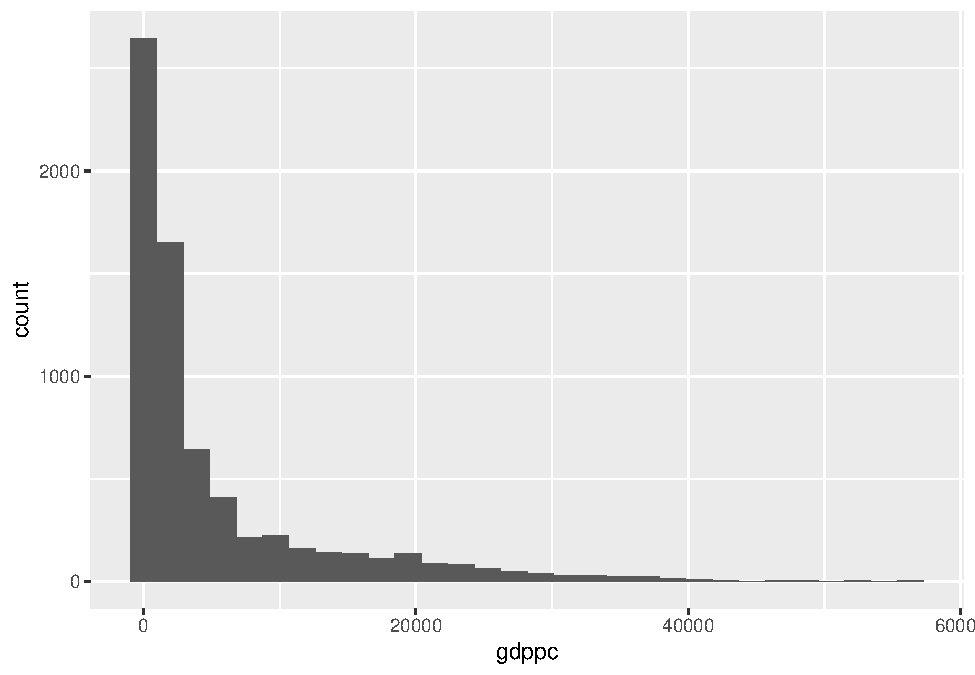
\includegraphics[keepaspectratio]{week2_files/figure-latex/unnamed-chunk-10-1.pdf}}

\subsection{Question 8: Comparing income by
regime}\label{question-8-comparing-income-by-regime}

The plot above is showing the distribution of income for both
democracies and autocracies together. Pass the argument
\texttt{fill\ =\ dem\_label} to the \texttt{aes()} to see how the
distributions differ by political regime. From this plot, can you tell
if democracies are richer or poorer than autocracies?

\subsection{Answer 8}\label{answer-8}

\begin{Shaded}
\begin{Highlighting}[]
\FunctionTok{ggplot}\NormalTok{(anrr, }\FunctionTok{aes}\NormalTok{(}\AttributeTok{x=}\NormalTok{gdppc, }\AttributeTok{fill =}\NormalTok{ dem\_label)) }\SpecialCharTok{+}
  \FunctionTok{geom\_histogram}\NormalTok{()}
\end{Highlighting}
\end{Shaded}

\pandocbounded{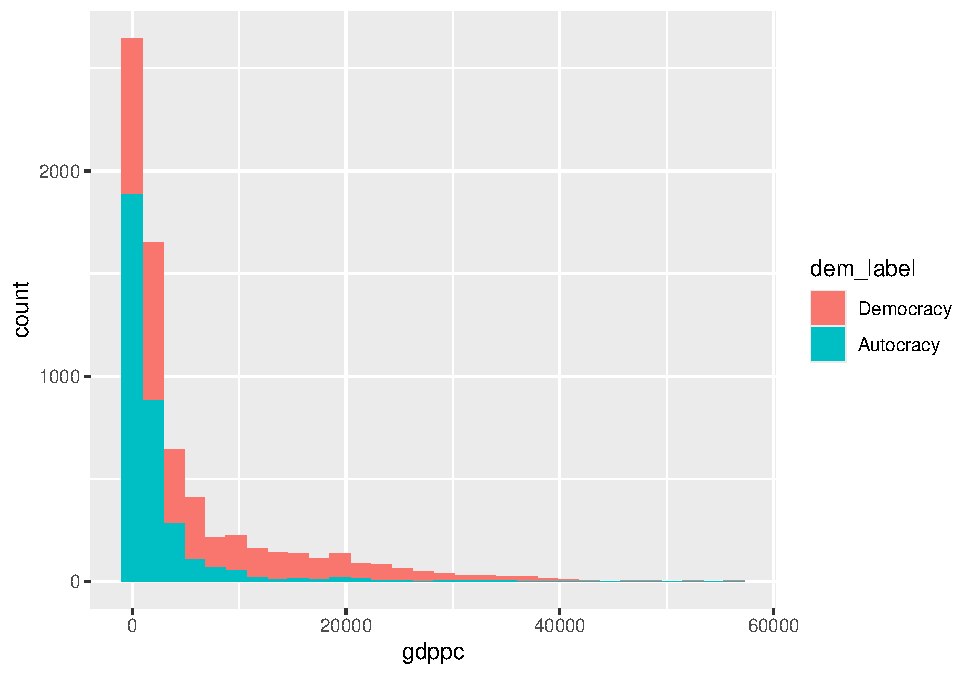
\includegraphics[keepaspectratio]{week2_files/figure-latex/unnamed-chunk-11-1.pdf}}

\subsection{Question 9: Log scale}\label{question-9-log-scale}

When the distribution of our variable is highly skewed, we often
transform the variable by a logarithmic scale. Make the same plot as in
2 above, but adding \texttt{scale\_x\_log10(labels\ =\ scales::dollar)}
as an argument to the \texttt{ggplot}. Does this transformation makes
clearer the income differences between democracies and autocracies?

\subsection{Answer 9}\label{answer-9}

\begin{Shaded}
\begin{Highlighting}[]
\FunctionTok{ggplot}\NormalTok{(anrr, }\FunctionTok{aes}\NormalTok{(}\AttributeTok{x=}\NormalTok{gdppc, }\AttributeTok{fill =}\NormalTok{ dem\_label)) }\SpecialCharTok{+}
  \FunctionTok{geom\_histogram}\NormalTok{() }\SpecialCharTok{+}
  \FunctionTok{scale\_x\_log10}\NormalTok{(}\AttributeTok{labels =}\NormalTok{ scales}\SpecialCharTok{::}\NormalTok{dollar)}
\end{Highlighting}
\end{Shaded}

\pandocbounded{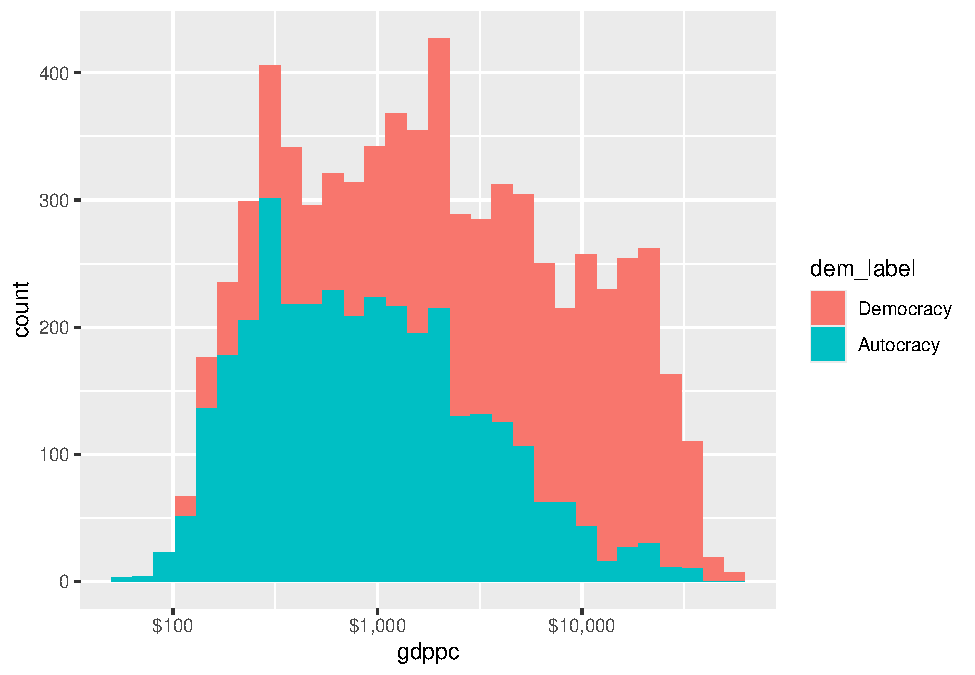
\includegraphics[keepaspectratio]{week2_files/figure-latex/unnamed-chunk-12-1.pdf}}

\subsection{Question 10: Comparing with
boxplot}\label{question-10-comparing-with-boxplot}

An alternative way to get to the question is to compare the median
income between political regimes. We can do this using
\texttt{geom\_boxplot}. What does this plot tells you about the
distribution of income in democracies when compared to autocracies?

\subsection{Answer 10}\label{answer-10}

\begin{Shaded}
\begin{Highlighting}[]
\FunctionTok{ggplot}\NormalTok{(anrr, }\FunctionTok{aes}\NormalTok{(}\AttributeTok{x=}\NormalTok{dem\_label, }\AttributeTok{y=}\NormalTok{gdppc)) }\SpecialCharTok{+} 
  \FunctionTok{geom\_boxplot}\NormalTok{() }\SpecialCharTok{+}
  \FunctionTok{scale\_y\_log10}\NormalTok{(}\AttributeTok{labels =}\NormalTok{ scales}\SpecialCharTok{::}\NormalTok{dollar)}
\end{Highlighting}
\end{Shaded}

\pandocbounded{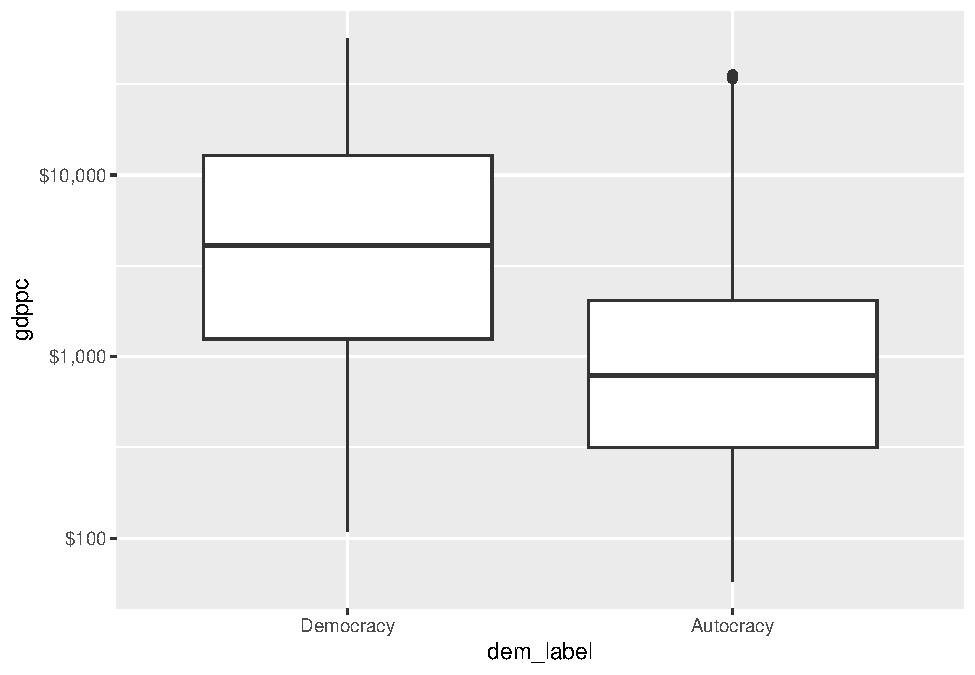
\includegraphics[keepaspectratio]{week2_files/figure-latex/unnamed-chunk-13-1.pdf}}

\subsection{Question 11: Comparing by country
groups}\label{question-11-comparing-by-country-groups}

Finally, do these patterns vary by world region? Add
\texttt{facet\_wrap(\textasciitilde{}region)} to your \texttt{ggplot} to
see the division by geographic/economic region. Region acronyms are AFR:
Africa , EAP: East Asia and the Pacific, ECA: Europe and Central Asia,
INL: OECD and high income countries, LAC: Latin America and Caribbean,
MNA: Middle East and North Africa, SAS: South Asia. Can you find a
region of the world where the median income of autocracies is higher
than that of democracies?

\subsection{Answer 11}\label{answer-11}

\begin{Shaded}
\begin{Highlighting}[]
\FunctionTok{ggplot}\NormalTok{(anrr, }\FunctionTok{aes}\NormalTok{(}\AttributeTok{x=}\NormalTok{gdppc, }\AttributeTok{fill =}\NormalTok{ dem\_label)) }\SpecialCharTok{+}
  \FunctionTok{geom\_boxplot}\NormalTok{() }\SpecialCharTok{+}
  \FunctionTok{scale\_x\_log10}\NormalTok{(}\AttributeTok{labels =}\NormalTok{ scales}\SpecialCharTok{::}\NormalTok{dollar) }\SpecialCharTok{+}
  \FunctionTok{facet\_wrap}\NormalTok{(}\SpecialCharTok{\textasciitilde{}}\NormalTok{region)}
\end{Highlighting}
\end{Shaded}

\pandocbounded{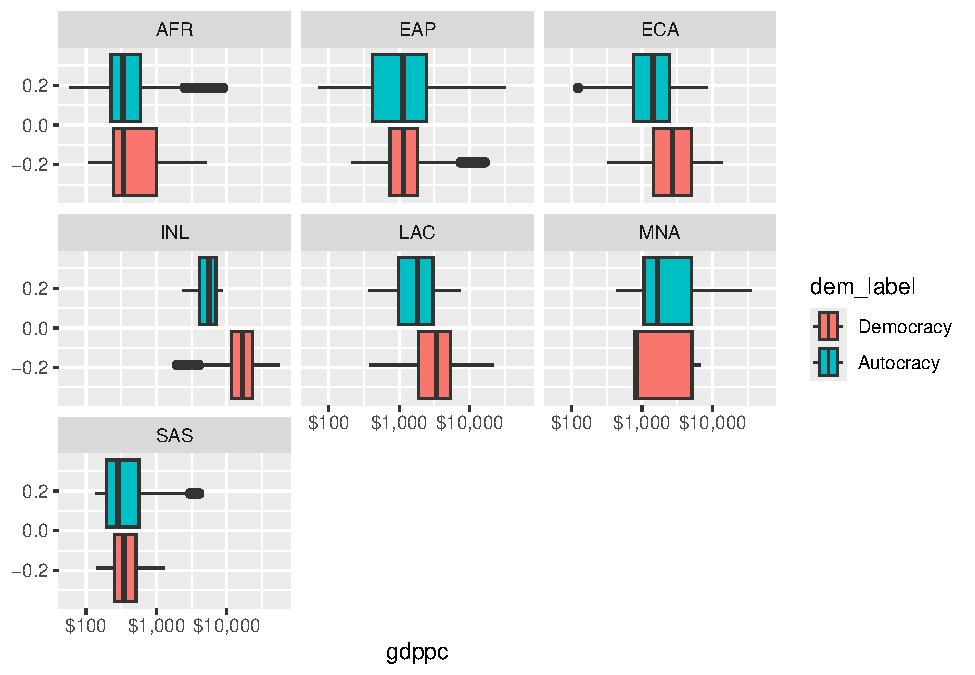
\includegraphics[keepaspectratio]{week2_files/figure-latex/unnamed-chunk-14-1.pdf}}

\end{document}
